%-------------------------------------------------------------------------------
\section{Preliminary Results}
%-------------------------------------------------------------------------------

\begin{figure*}[t!]
    \centering
      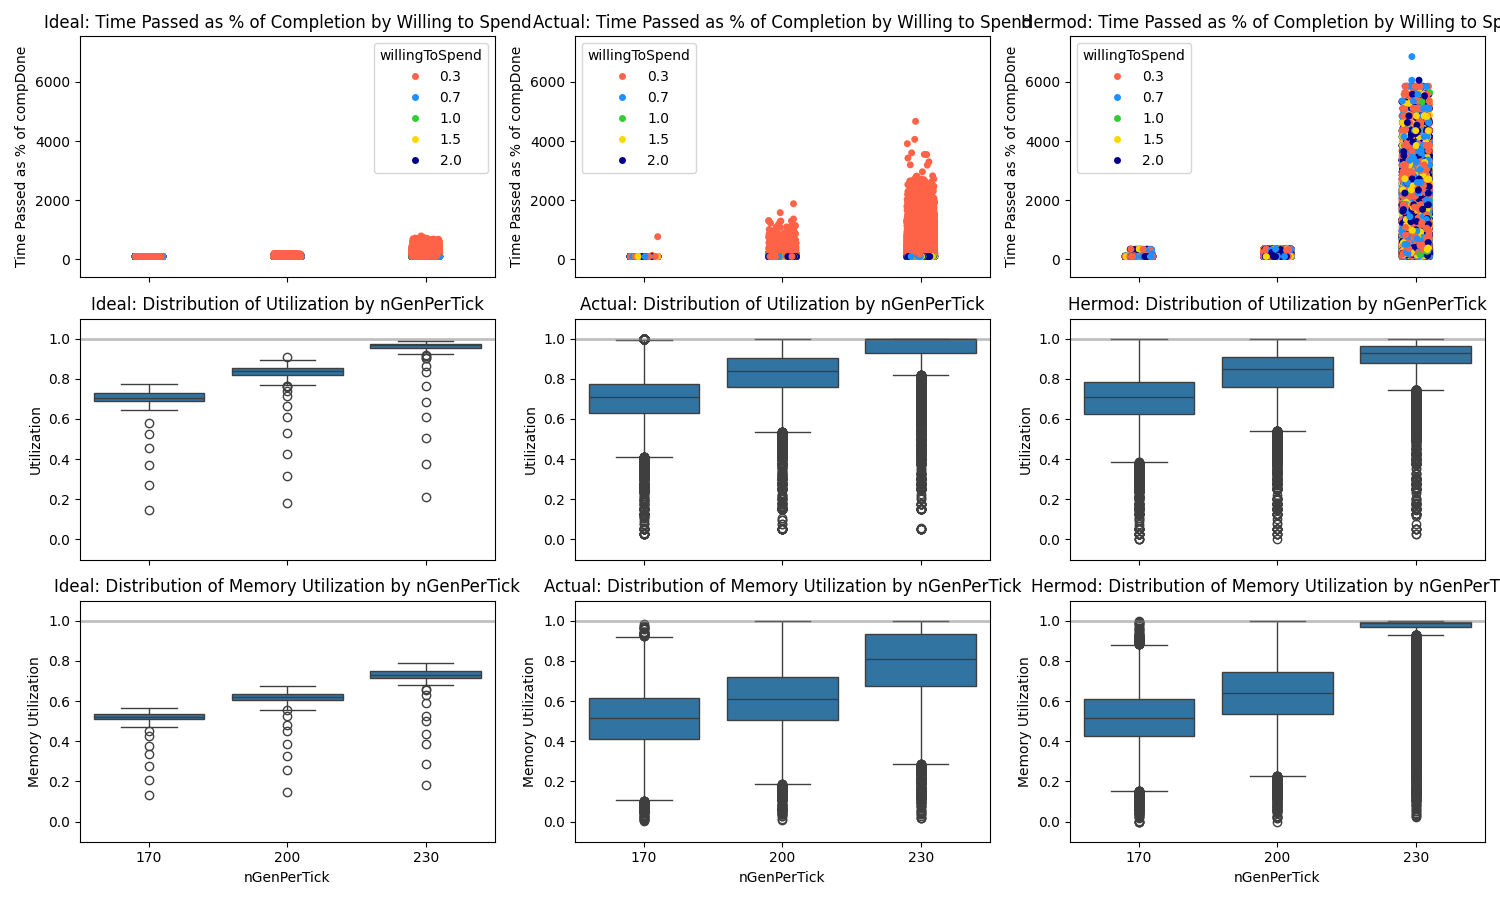
\includegraphics[width=15cm]{img/combined_res.png}
      \caption{ a first version of the graph }
    \label{fig:graph}
\end{figure*}

To understand the dyanmics of \sys{}, we built a simulator in go\cite{TODO}. Our
simulator runs three different worlds: an ideal scheduling world, an
implementation of \sys{}'s design, and an implementation of Hermod\cite{TODO}. 

The idealized scheduler runs in a centralized setting: it is as if the whole
datacenter is one machine with many many cores. As such there is no memory
fragmentation, and its utilization represents an optimal solution. It still has
the same limited memory as the datacenter though, so will kill using the same
mechanism as \sys{}.\hmng{not sure if this is clear and I should just shut up or
if it's non-obvious and I should explain it more}

Hermod is a scheduler built specifically for serverless, and is the result of a
from-first-principles analysis of different scheduling paradigms through a
simulator. The paper simulates different scheduling approaches along three
dimensions: late-vs early binding; Processor Sharing (PS) vs First Come First
Served (FCFS) vs (idealized) Shortest Remaining Processing Time (SRPT); and
least loaded vs locality based vs random load balancing. The paper concludes
that early binding is best, in combination with PS (PS is close enough to SRPT
with perfect knowledge, which is impractical in reality). For the load balancing
Hermod uses a hybrid mechanism: at low load, Hermod packs machines one by one,
each up until the number of cores (a water-filling like mechanism, where each
machine is filled until each core is running a job); and at high load it chooses
the least loaded machine. Hermod does not use priorities in its design, and as
such we ignore jobs' priority when placing them in the Hermod world in our
simulator.


In the simulator, jobs arrive in an open loop at a constant rate. The simulator
attaches three main characteristics to each job it generates: runtime, priority,
and maximum memory usage.\ \textit{Job runtime} is chosen by sampling from
randomly generated long tailed (in this case pareto) distribution: the relative
length of the tail ($\alpha$ value) remains constant, and the minimum value
($x_m$) is chosen from a normal distribution. This reflects the fact that
different functions have different expected runtimes (chosen from a normal
distribution), and that actual job runtimes follow long tailed distributions (so
each pareto distribution that we sample represents the expected runtime
distribution of a given function).\ \textit{Job priority} is chosen randomly. The
simulator has five different priority values, each assigned to the prices of 3c,
7c, 10c, 15c, 20c.\hmng{does it matter that these prices are unrealistic}
Because functions are randomly assigned a priority, runtime and priority are not
correlated.\ \textit{Maximum memory} is chosen uniform random between 1MB and
10GB.

The simulator makes some simplifying assumptions:
\begin{enumerate}
    \item functions are compute bound, and do not block for i/o
    \item functions use all of their memory right away
    \item communication latencies are not simulated
\end{enumerate}


We then run the simulator at different load points, and track latencies as a
percentage of the required runtime, as well as memory and compute utilization;
for each of the three different worlds of \sys{}, Hermod, and ideal.

A good result for \sys{} would be doing in between Hermod and the ideal world.
We expect \sys{} will do better than Hermod because it has more knowledge:
whereas Hermod will spread latency hits across all jobs indiscriminately as load
goes up, \sys{} can keep high priority jobs running quickly and limit the
slowdown to only affect lower priority jobs. We cannot expect \sys{} to do as
well as the ideal world: not only does \sys{} have to deal with memory
fragmentation, which the ideal world does not, but it also has imperfect
information --- once the idle list is empty, \sys{} relies on k choices to find
a fitting machine. 

We see the results of a run in Figure \ref{fig:graph}. As expected, \sys{} does
not perform as well as the ideal world: latencies rise more quickly, and both
compute and memory utilization have a higher variance across machines and time.
We can also see that, as expected, under higher load \sys{} is able to keep all
priorities except the lowest running with low latency, whereas Hermod slows down
all the functions the same.


